\documentclass{article}
\usepackage[margin=0.5in]{geometry}
\usepackage{textcomp}
\usepackage{pgfplots}
\pgfplotsset{width=10cm,compat=1.9}

\begin{document}

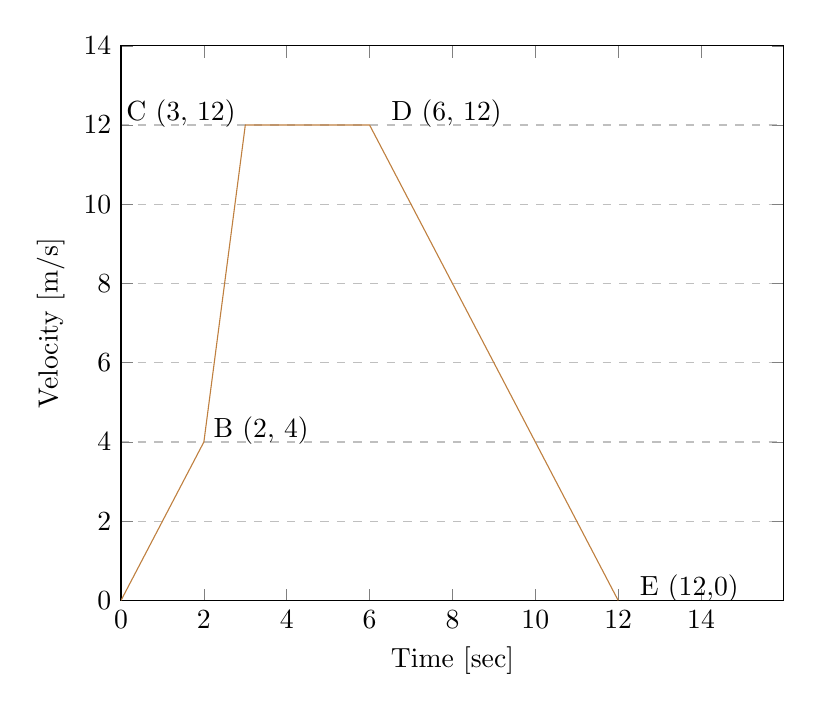
\begin{tikzpicture}
\begin{axis}[
    xlabel={Time [sec]},
    ylabel={Velocity [m/s]},
    xmin=0, xmax=16,
    ymin=0, ymax=14,
    xtick={0, 2, 4, 6, 8, 10, 12, 14},
    ytick={0, 2, 4, 6, 8, 10, 12, 14},
    legend pos=north west,
    ymajorgrids=true,
    grid style=dashed,
]

\addplot[
    color=brown,
    ]
    coordinates {
    (0,0) (2,4)(3,12)(6,12)(12,0)
    
    };
\node[above left, xshift=1ex, yshift=-1ex] at (axis cs:0,0) {A};
\node[above right, xshift=0ex, yshift=-1ex] at (axis cs:2,4) {B (2, 4)};
\node[above left, xshift=0ex, yshift=-1ex] at (axis cs:3,12) {C (3, 12)};
\node[above right, xshift=1ex, yshift=-1ex] at (axis cs:6,12) {D (6, 12)};
\node[above right, xshift=1ex, yshift=-1ex] at (axis cs:12,0) {E (12,0)};
\end{axis}
\end{tikzpicture}
\end{document}